\chapter{Attacker's View of Active Directory}

\textbf{Defender's Dilemma:}
\begin{itemize}
    \item Attacker just need to win once
    \item Defenders need to win all the time
    \end{itemize}

    \textbf{Attacker's Dilemma:}
    \begin{itemize}
        \item Attackers need to evade all detection
        \item Defenders just need on alarm or trigger to know attackers are in
        \item "Defender's Dilemma vs. Intruder's Dilemma" - Tao Security (2009)
    \end{itemize}

\section{Assume Breach}

\subsection{Assume Breach Mentality}
\begin{itemize}
    \item Prepare for threats beyond the Wall (Defense in Depth / Layered Defense Security) - CYBER RESILIENCE
    \item Detect and Respond to threats (Threat Hunting / IOC) - CYBER AGILITY
    \item Prevention is still important but critical to move beyond it

\end{itemize}

\subsection{Adversarial Tactics, Techniques, and Common Knowledge (ATT\&CK)}

\begin{figure}
    \centering
    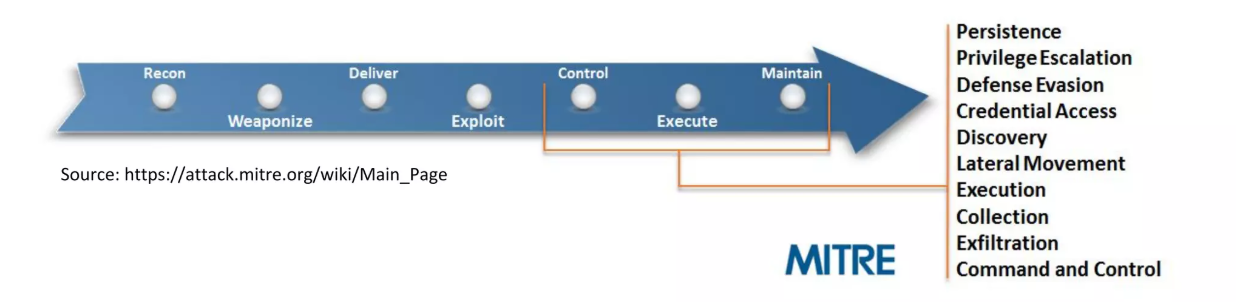
\includegraphics[width=0.75\linewidth]{mitreattack.png}
    \caption{Red Team Tactics, Techniques, and Procedures (TTPs)}
    \label{fig:placeholder}
\end{figure}

\subsection{Active Directory}
\begin{itemize}
    \item Active Directory Domain Services (AD DS)-A set of services to manage network resources.
    \item Domain Controller (DC)-Server running AD DS.
    \item Domain Admin (DA)-The privileged user group that has full control of network resources in the domain.
    \item  Local Administrators-The privileged user group that has full control for resources contained within the local machine.
\end{itemize}

\subsection{Windows Authentication Types}
\begin{itemize}
    \item NTLM Authentication
    \begin{itemize}
        \item Challenge-Response Protocol
    \end{itemize}
\item Kerberos
\item Single Sign-On (SSO)
\end{itemize}

\subsection{NTLM Authentication}
\begin{figure}
    \centering
    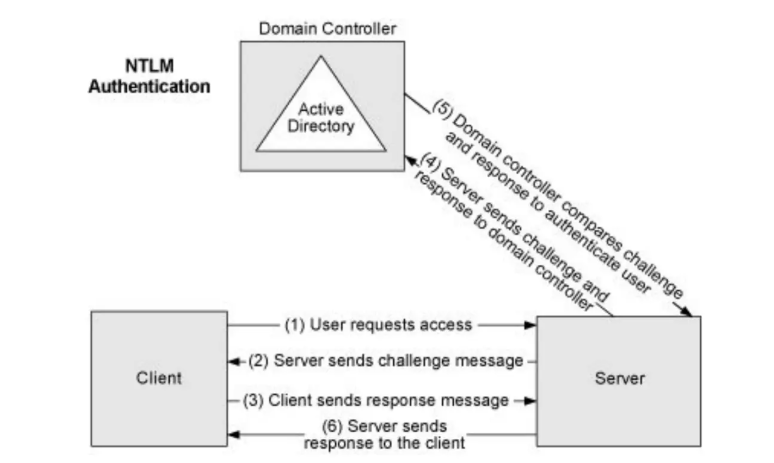
\includegraphics[width=0.75\linewidth]{ntlmauth.png}
    \caption{NTLM Authentication}
    \label{fig:placeholder}
\end{figure}

\subsection{Kerberos Authentication}
\begin{figure}
    \centering
    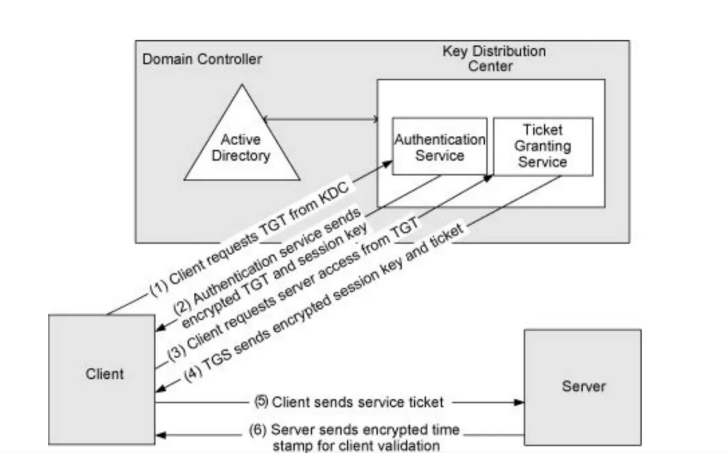
\includegraphics[width=0.75\linewidth]{kerberosauth.png}
    \caption{Kerberos Authentication}
    \label{fig:placeholder}
\end{figure}
\begin{itemize}
    \item \textbf{Ticket Granting Ticket (TGT) contains:}
    \begin{itemize}
        \item Privilege Attribute Certificate (PAC) stores
        \begin{itemize}
            \item Account Name
            \item Security Identifiers (SIDs)
            \item Group Membership
        \end{itemize}
    \end{itemize}
\item User requests for TGT by sending timestamp that is encrypted with user's secret key (NTLM Hash for RC4 Cipher / RC4 HMAC Hash)
\item TGT is encrypted and its PAC is signed by the domain account \texttt{krbtgt's} secret key (NTLM Hash)-Only readable by Domain Controllers (DCs)
\item Service ticket issued by Ticket Granting Service (TGS) is encrypted by service account's secret key (NTLM Hash)
\end{itemize}

\subsection{High Level Methodology}
\begin{figure}
    \centering
    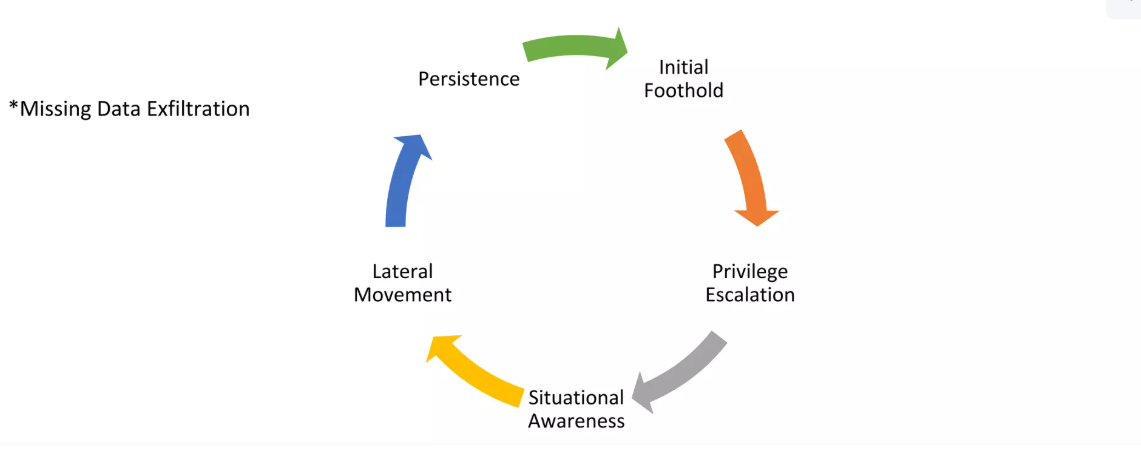
\includegraphics[width=0.75\linewidth]{highlevel.png}
    \caption{High Level Methodology}
    \label{fig:placeholder}
\end{figure}

\subsection{Initial Toehold}
\begin{itemize}
    \item Unpatched Vulnerabilities
    \item Spearphishing
    \item Weak Credentials
\end{itemize}

\subsection{Privilege Escalation: Use to Local Admin}
\begin{itemize}
    \item Unpatched Vulnerabilities
    \item System Misconfigurations
    \begin{itemize}
        \item Passwords stored in \texttt{SYSVOL} or Group Policy Preference (GPP)
    \end{itemize}
\end{itemize}

\subsection{Passwords Stored in \texttt{SYSVOL}}
\begin{itemize}
    \item \texttt{SYSVOL}
    \begin{itemize}
        \item Domain-wide shared folder
        \item Stores logon scripts, domain group policies
        \item Any authenticated user on the domain can access it
    \end{itemize}
\item Scripts with cleartext admin credentials are stored in \texttt{SYSVOL}
\item Group Policy with password defined for Local Administrator account:
\begin{figure}
    \centering
    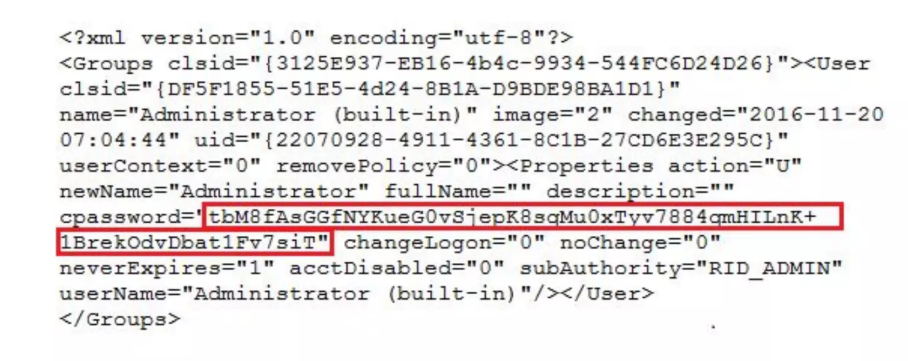
\includegraphics[width=0.75\linewidth]{adminpwd.png}
    \caption{Local administrator account password hash}
    \label{fig:placeholder}
\end{figure}
\end{itemize}
\begin{itemize}
    \item Encryption is well-known
    \item All passwords are encrypted using a derived Advanced Encryption Standard (AES) key
    \item The 32-byte key is as follows:
\begin{figure}
    \centering
    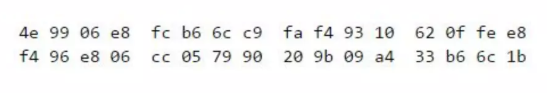
\includegraphics[width=0.75\linewidth]{aes.png}
    \caption{32-byte AES encryption key}
    \label{fig:placeholder}
\end{figure}
\end{itemize}
\begin{itemize}
    \item Once the hash is cracked offline, the plaintext administrative passwords is revealed:
    \item 
\begin{figure}
    \centering
    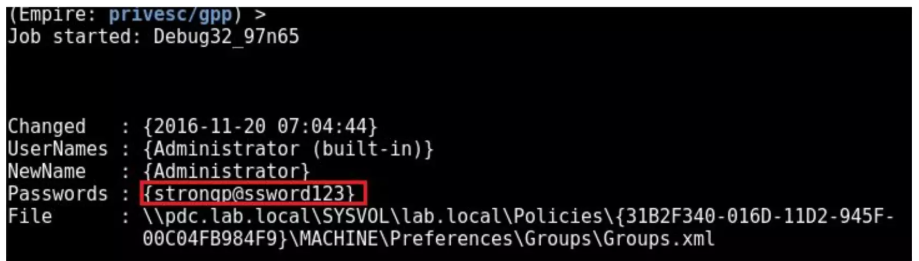
\includegraphics[width=0.75\linewidth]{crackedpwd.png}
    \caption{Cracked plaintext administrative password}
    \label{fig:placeholder}
\end{figure}
\end{itemize}
\subsection{Passwords Stored in \texttt{SYSVOL} Mitigation\& Detection}
\begin{itemize}
    \item Install KB2962486 to disable new credentials from being stored in GPP and delete existing XMLs / Group Policies
    \item Plant an XML file with "Password" in \texttt{SYSVOL}
    \item Configure SACL on the XML to audit for access
\end{itemize}

\subsection{Why We Need Privilege Escalation}
\begin{itemize}
    \item Gain access to implicit trust relationship artifacts
    \item Assume artifacts found on one machine could be used to access other machines
\end{itemize}

\subsection{Dump Implicit Trust Relationship Artifacts}
\begin{itemize}
    \item Dump and crack local account hashes (Hashes == Password)
    \item Dump credentials stored in-memory
    \item Dump Kerberos tickets
    \item Dump access tokens
\end{itemize}

\subsection{Dump Credentials In-Memory Using Mimikatz}
\begin{figure}
    \centering
    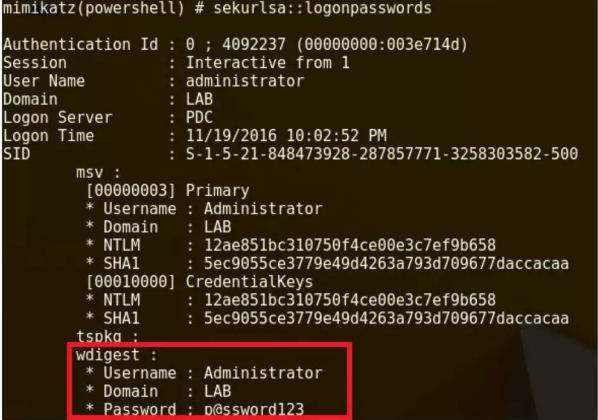
\includegraphics[width=0.75\linewidth]{mimikatz.png}
    \caption{In-memory credential dump using Mimikatz tool}
    \label{fig:placeholder}
\end{figure}
\subsection{Dump Credentials Mitigation}
\begin{itemize}
    \item Audit for misconfigurations that can lead to privilege escalation with \texttt{'windows-privesc-check'}
    \item Install KB2871997 on Windows 7/8/10/11 and on Windows Server 2008/2012/2019
    \item Deploy Application Allowlisting (AppLocker \& Device Guard)
    \item Get rid of Windows Server 2003 completely
    \item Incorporate PAWs and SAWs (Privileged / Secured Administrative Workstations) as Domain Admins should not be logging on to machines with lower trust levels (e.g., a norml end-user workstation or laptop).
\end{itemize}

\subsection{Dump Credentials Detection}
    \begin{itemize}
    \item Monitor Registry Value for \texttt{"UseLogonCredential"} at 
    \texttt{HKEY\_LOCAL\_MACHINE\textbackslash SYSTEM\textbackslash CurrentControlSet\textbackslash Control\textbackslash SecurityProviders\textbackslash Wdigest}
    \item Value: \texttt{"1"} to enable cleartext passwords to be stred in LSASS
    \item Honey Credentials
\end{itemize}

\subsection{Dump Credentials Detection (Not a Good Idea)}
\begin{itemize}
    \item Detect Mimikatz in-memory using \texttt{SYSMON} (be careful of performance impact)
    \item Look for loading of:
\end{itemize}
    \begin{itemize}
        \item \texttt{C:\textbackslash System32\textbackslash WinSCard.dll}
        \item \texttt{C:\textbackslash System32\textbackslash cryptdll.dll}
        \item \texttt{C:\textbackslash System32\textbackslash hid.dll}
    \end{itemize}
            \begin{itemize}
                \item     \texttt{C:\textbackslash System32\textbackslash WinSCard.dll}
            \end{itemize}
            \begin{itemize}
                \item \texttt{C:\textbackslash System32\textbackslash cryptdll.dll}
            \end{itemize}
            \begin{itemize}
                \item \texttt{C:\textbackslash System32\textbackslash hid.dll}
            \end{itemize}
            \begin{itemize}
                \item \texttt{C:\textbackslash System32\textbackslash samlib.dll}
            \end{itemize}
            \begin{itemize}
                \item \texttt{C:\textbackslash System32\textbackslash vaultcli.dll}
            \end{itemize}
\item LSA Protection Enabled-\texttt{mimidrv.sys} (Mimikatz's driver to turn off LSA Protection)
\end{itemize}

\subsection{User Access Control (UAC) Bypass}
\begin{itemize}
    \item Old School
    \begin{itemize}
        \item Privilege File Copy (File Operation COM)
        \item DLL Hijacking
        \item Auto-elevation
    \end{itemize}
\item New School
\begin{itemize}
    \item Fileless UAC Bypass via Registry Hijacking
    \item Write to \texttt{HKCU:\textbackslash SOFTWARE\textbackslash Classes\textbackslash mscfile\textbackslash shell\textbackslash open\textbackslash command.dll}
    \item Launch \texttt{eventvwr.exe}
\end{itemize}
\end{itemize}
\begin{figure}
    \centering
    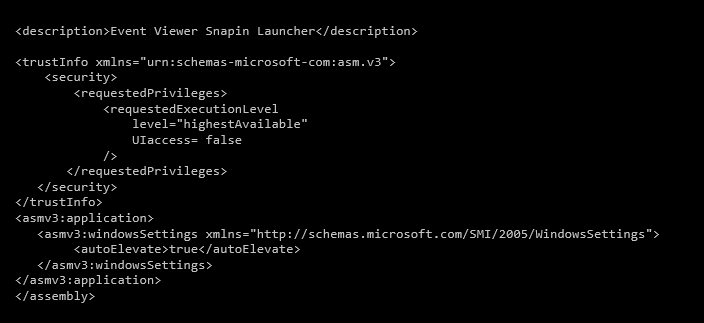
\includegraphics[width=0.75\linewidth]{eventvwr.png}
    \caption{Enter Caption}
    \label{fig:placeholder}
\end{figure}
\subsection{UAC Bypass Mitigation\& Detection}
\begin{itemize}
    \item Reduce users with administrative privileges
    \item Set UAC level to "Always Notify" instead of default configuration bypassed with Disk Clean up
    \item Monitor Registry entry:\texttt{"HKCU\textbackslash SOFTWARE\textbackslash Classes\textbackslash mscfile\textbackslash shell\textbackslash open\textbackslash command"}
\end{itemize}

\subsection{Situational Awareness}
\begin{itemize}
    \item Port Scan
    \item DNS Enumeration (\texttt{SRV records, *.\_tcp.domain.com})
    % \item Password / Hash Spray (commented out for debugging math mode error)
    \item Service Principal Name (SPN) Scanning
    \item Domain Enumeration and Admin Hunting
    \item BloodHound
\end{itemize}

\subsection{Password / Hash Spray}
\begin{itemize}
    \item Quick and dirty way to identify access across the network
    \item Good for pentests that do not require stealth
\end{itemize}
\begin{figure}
    \centering
    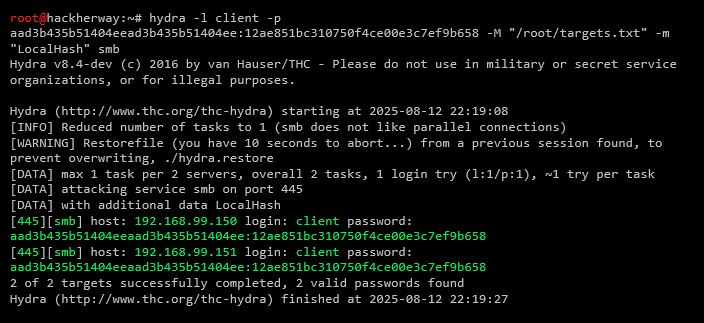
\includegraphics[width=0.75\linewidth]{spray.png}
    \caption{Password / Hash Spray}
    \label{fig:placeholder}
\end{figure}
\subsection{Service Principal Name (SPN) Scanning}
\begin{itemize}
    \item SPN is used to uniquely identify service instances for Kerberos authentication
    \item Gathers services across the domain (without a single port scanned)
\end{itemize}
\begin{figure}
    \centering
    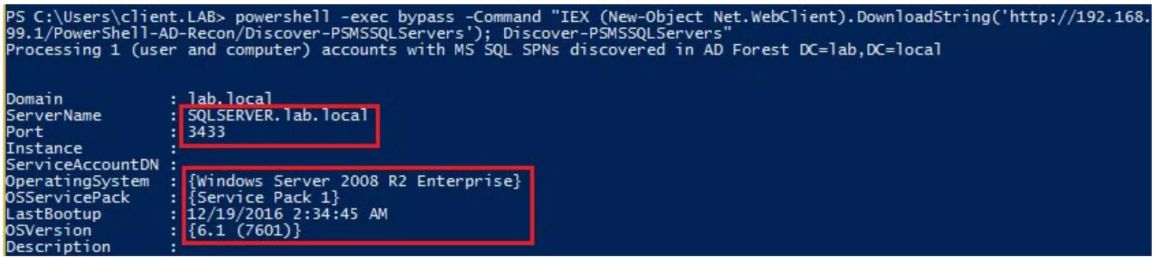
\includegraphics[width=0.75\linewidth]{spnscan.png}
    \caption{SPN scan}
    \label{fig:placeholder}
\end{figure}
\subsection{Domain Enumeration}
\begin{figure}
    \centering
    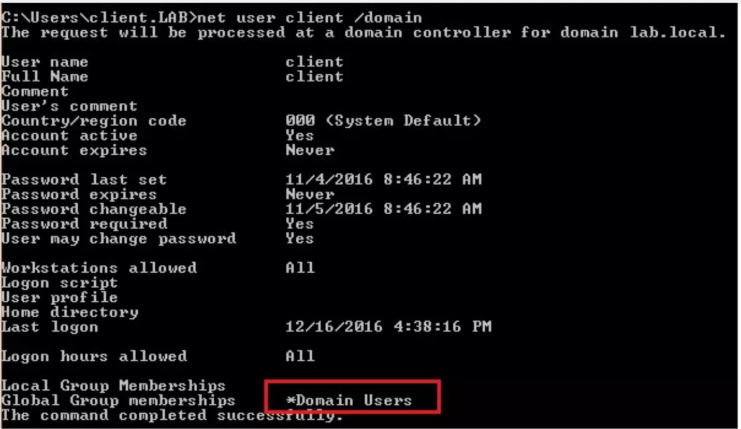
\includegraphics[width=0.75\linewidth]{domenum1.png}
    \caption{Domain user enumeration}
    \label{fig:placeholder}
\end{figure}
\begin{figure}
    \centering
    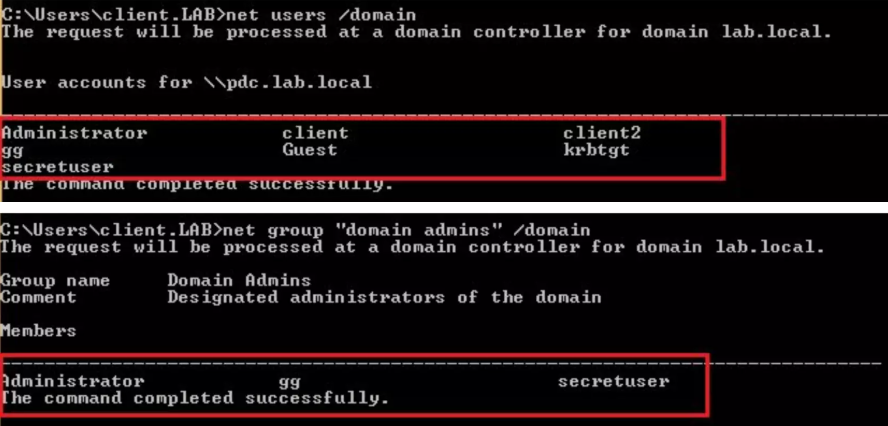
\includegraphics[width=0.75\linewidth]{domenum2.png}
    \caption{Domain Admin enumeration}
    \label{fig:placeholder}
\end{figure}
\subsection{Domain Enumeration with PowerView}
\begin{itemize}
    \item PowerView
    \begin{itemize}
        \item Based on PowerShell
        \item Capitalize on PowerShell alternatives for \texttt{"NET"} command 
        \item    Capitalize on Win32 API
        \item Gain network situational awareness
\end{itemize}
\end{itemize}
\begin{figure}
    \centering
    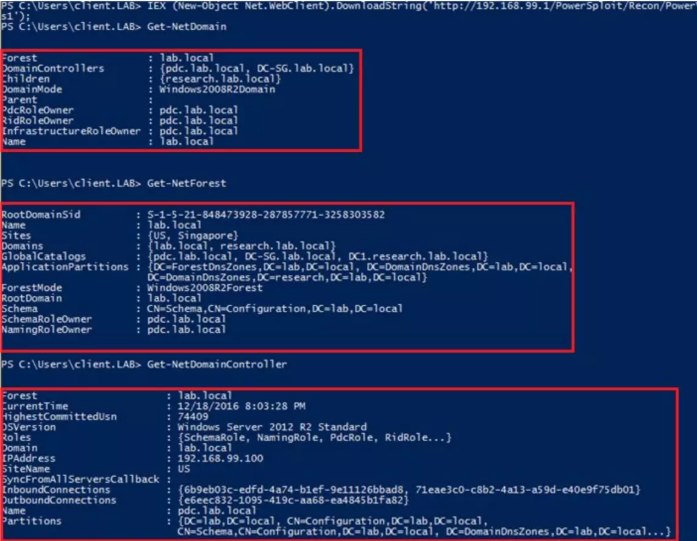
\includegraphics[width=0.75\linewidth]{pv1.png}
    \caption{Domain enumeration using the PowerView tool}
    \label{fig:placeholder}
\end{figure}
\begin{figure}
    \centering
    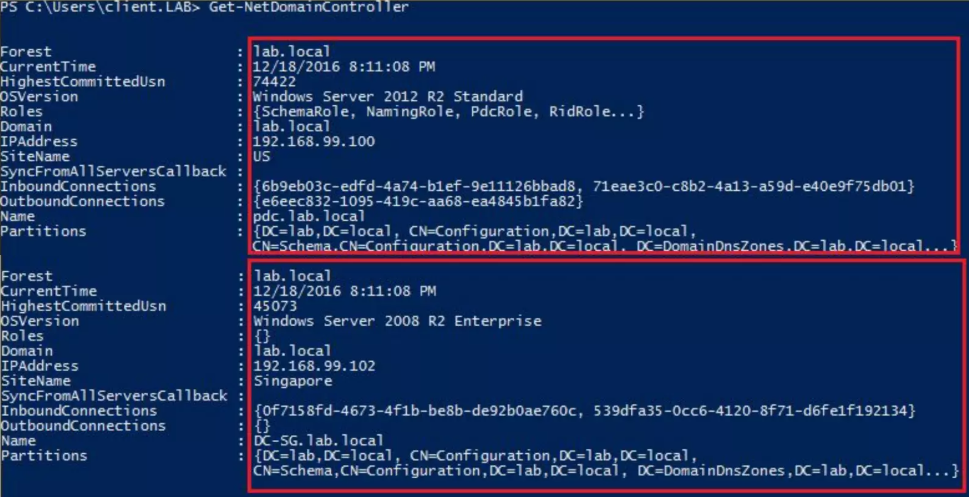
\includegraphics[width=0.75\linewidth]{domenum3.png}
    \caption{Domain Controller (DC) enumeration using the PowerView tool}
    \label{fig:placeholder}
\end{figure}
\begin{figure}
    \centering
    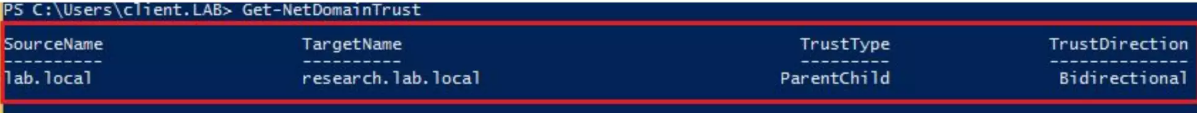
\includegraphics[width=0.75\linewidth]{trustenum.png}
    \caption{Domain trust enumeration using the PowerView tool}
    \label{fig:placeholder}
\end{figure}
\subsection{Admin Hunting with PowerView}
\begin{itemize}
    \item Implicit trust relationship
    \item Look at where the current user has Local Administrator Right
    \item Look for where privileged users are logged on to
    \item Target machines with privileged users
    \item Steal their tokens / credentials
    \item Profit
\end{itemize}

\subsection{Admin Hunting with PowerView Commands}
\begin{itemize}
    \item \texttt{Invoke-UserHunter}
    \begin{itemize}
        \item Get a list of hosts from AD
        \item Get a list of users of a specific Domain Group (Domain Admins / Local Administrator)
        \item Run \texttt{NetSessionEnum} (User Sessions) and \texttt{NetWkstaUserNum} (Logged On Users with information gathered)
        \item (Optionally) Check if current user has :Local Administrators rights on each host
    \end{itemize}
\end{itemize}











